\documentclass[12pt]{article}

\usepackage{siunitx} % Provides the \SI{}{} and \si{} command for typesetting SI units
\usepackage{amsmath} % Required for some math elements 
\usepackage[left=1in,top=1in,right=1in,bottom=1in]{geometry}
\usepackage[T1]{fontenc}
\usepackage[none]{hyphenat} %removes hyphentation
\usepackage{verbatim}
\setlength\parindent{24pt}
\usepackage{setspace}
%\pagenumbering{gobble} %removes page numbering
\usepackage{graphicx} %images
\usepackage{textcomp}
\usepackage{gensymb} %degree symbol
\graphicspath{{images/}}
\usepackage{etoolbox}
\usepackage{multicol}

\renewcommand{\baselinestretch}{1.15} 

\title{\vspace{-3em} \textbf{\Large Displaying local weather conditions through LEDs}}
\author{Justin Kang \\ CS 378: Autonomous Intelligent Robotics (FRI)}
\date{May 12, 2016}

\begin{document}
\maketitle
%\doublespace


\section*{Abstract} 
The goal of the project was to create a method of displaying local weather conditions on the robots in the UT CS Department's segbots, specifically through the use of communication between a ROS node and an Arduino connected to Pololu LEDs. Specifically, this resulted in the presentation of specifically the temperature in the Austin area. While the goal of the project was technically accomplished, there were some limitations that were faced in implementing the project and with possible expansions of the project, and currently exist within the source code. Various approaches for solutions for these limitations are discussed. Finally, while this project was a useful venture, the main potential of this project lies within future extensions. These possibilities are discussed at the end of the paper.


\section{Introduction}
While this project may not be the most relevant project when considering the whole of the BWI project, this project merely seeks to provide a convenient and easy way to display weather data to those that are working in the building with these robots. Particularly when looking at the various possibilites for expansion on this project, this provides a very quick and easy way to present information to the users, as well as presenting a wide possible range of weather information. Considering the irregularity of the weather in Texas, especially in the spring and fall seasons, this project acts as a early-warning system in order to display these possible irregularities to the users, especially when such information can easily be forgotten, or never encountered in the first place.


\begin{figure}[ht]
\centering
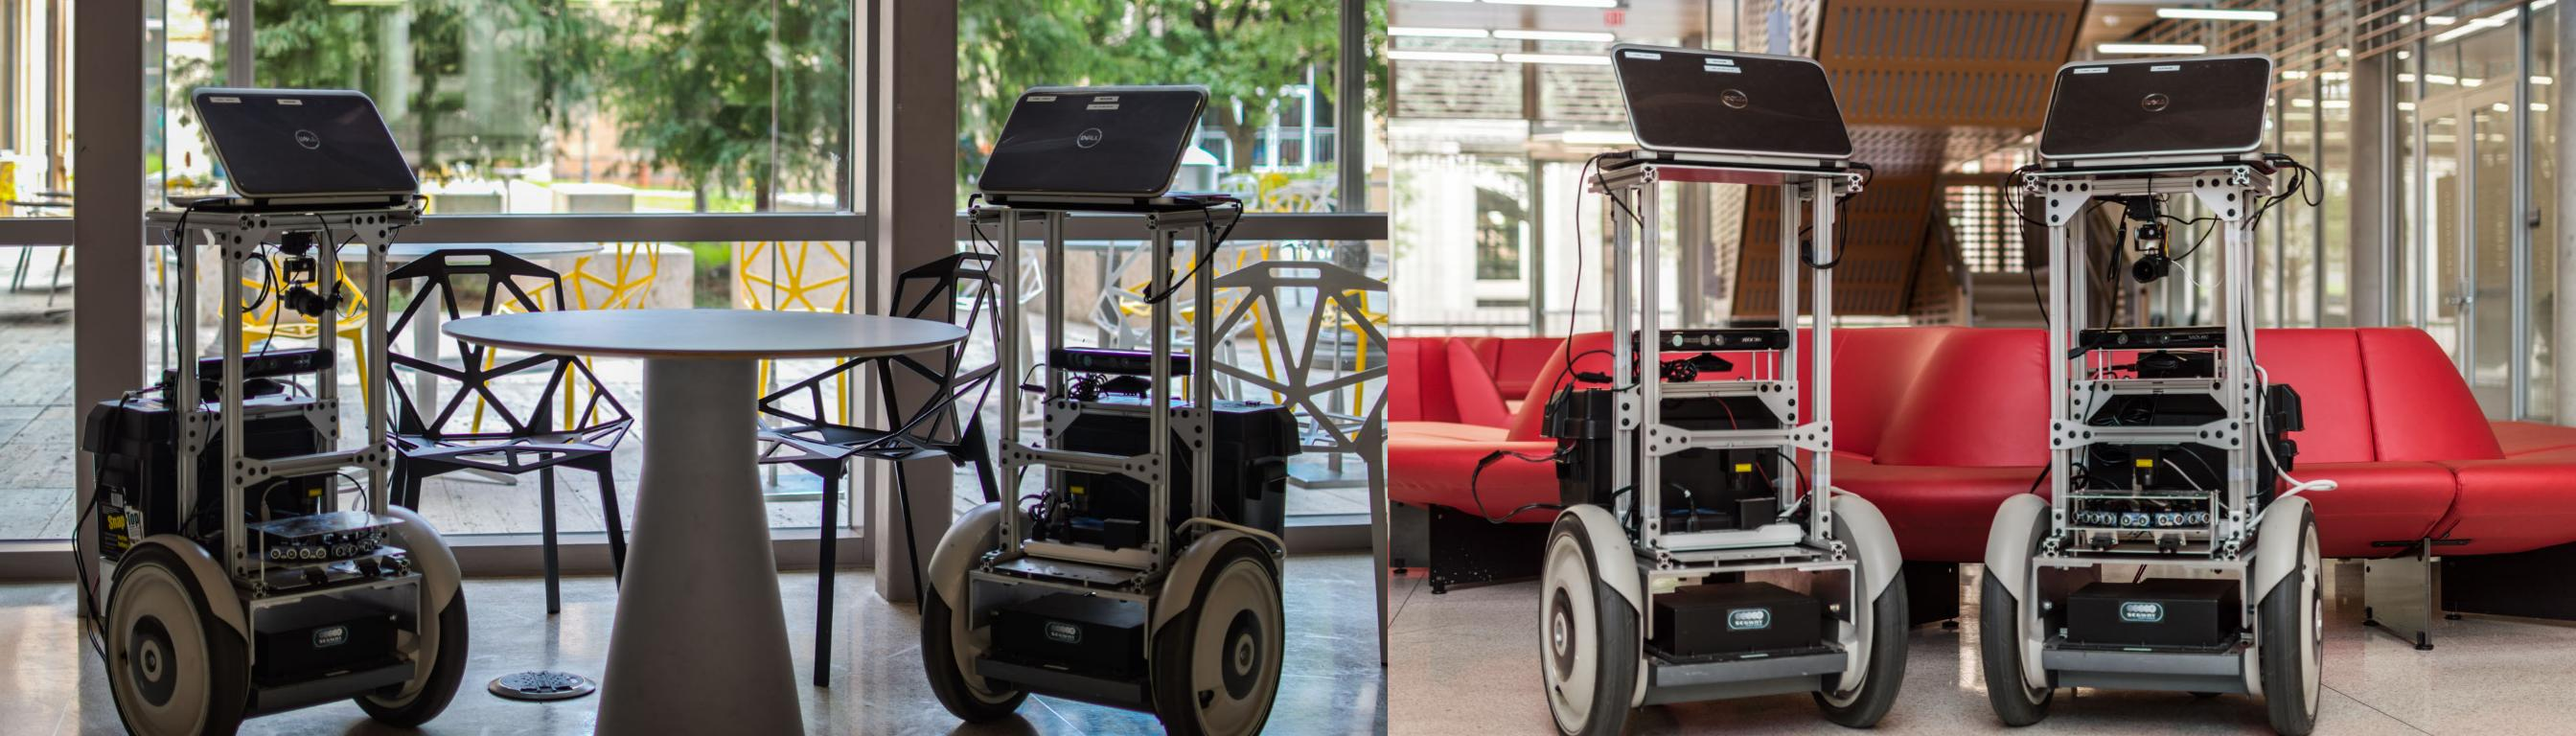
\includegraphics[height=0.3\textwidth, width=\textwidth]{Segbot.jpg}
\caption{The segbots at the University of Texas at Austin [1]}
\end{figure}


\section{Background Information}
This project makes use of communication between a Python script and an Arduino. The script obtains the weather by requesting the information in the form of JSON through the Weather Underground API [3]. The script then goes through the JSON and stores the next x hours' worth of temperatures within a dictionary. In this case, twelve hours are used. \\\\ After obtaining all of the necessary information, the script then sends all of this information to the Arduino through serial communication. In this process, information is sent in bytes (or chars) from the script to the Arduino through a connection channel.\\
\indent The Arduino then picks up the work from here. First it reads all of the sent information from the serial communication, and then stores all of these in an array of ints. It then divides the temperature by 120, as the extremes of the temperatures in Texas are approximated to 0{\degree}F and 120{\degree}F. The temperature then is rescaled to a range of 0 to 255 so that it can be converted to the RGB scale. For this project, yellow was chosen as cold, while red was chosen as hot. These colors are then displayed on the Pololu LED strips attached to the segbots. Related projects include not necessarily anything involving current research within the field of computer science nor robotics, but rather applications of meteorology. Thus, the closest related projects are probably those involving how human perception translates colors and visual keys to other information, such as weather and temperature.\\
\indent Related works involve studies that investigate exactly how people interpret temperature based on colors, specifically in terms of what they think are considered as colder colors, and what are considered as warmer colors. In this case, these are drawn mostly from the fields geosciences and meteorology, rather than computer science. Other background information that may be useful are the examples provided by Pololu for their LEDs [4], serial communication, and server requests from code.


\begin{figure}[ht]
\centering
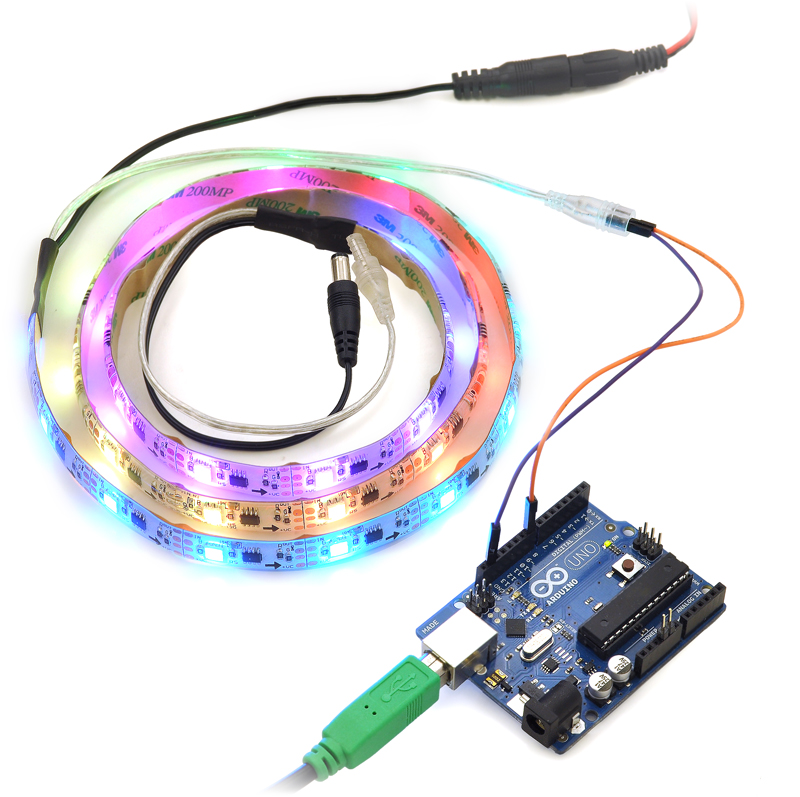
\includegraphics[height=0.4\textwidth, width=0.8\textwidth]{Pololu.jpg}
\caption{The Pololu LED strip [2]}
\vspace{-1em}
\end{figure}


\section{Technical Approach}

\subsection{Programming}
Most of the code for the Python script was obtained from David Wechsler and his blog [5]. Following the general template, I had to change the code so that rather than obtaining historical temperatures in St. Louis, I needed to obtain the weather forecast for Austin. \\\\ Furthermore, rather than returning the dictionary, I needed to be able to send these values to the Arduino over serial communication. This was done following the general outline that I found on stackoverflow [6].\\
\indent For the Arduino program, I followed the examples on Pololu's Github [4]. Rather than having predetermined values for the lights, the program reads the temperature values over serial, and uses those in order to determine what color to produce on the LEDs. I restricted this reading so that once the array of temperatures has been set, the Arduino program no longer attempts to read from serial, due to limitations caused by my Python code.

\subsection{Limitations}
As previously mentioned, there are several limitations within my code right now. The first three of these have to do with the Python code, the first being updating the forecast over time. As my current Python script only obtains the forecast from the moment it is run, it is unable to update the forecast, and thus LEDs as time passes. This can lead to the information presented on the LEDs being easily and quickly outdated (that is, in the span of just twelve hours). The second doesn't directly relate to code itself, but rather the API I am using. The Weather Underground API only allows for 500 free requests in a 24-hour period. Thus, I am unable to continuously send requests, as this would lead to quickly reaching the limit. Although there do exist alternatives that allow for an unlimited amount of requests, they trade away most of the information and functionality that the Weather Underground API allows for. Finally, the last limitation within my code is localization of the weather forecast. Currently the program is hard-coded to obtain information for Austin, and thus there is no option for the user to easily change the location as necessary.\\\\
\indent There are two clear limitations within the Arduino code, the first being the colors that are presented on the LEDs. Whereas I originally wanted to create a range between blue and red for the temperatures in order to simulate weather station reports, I was unable to find an easy way to scale this from temperature to RGB values. Thus I changed the scale to yellow to red for easy conversion; however this can be misleading as some may still perceive yellow to be fairly warm, even if it is supposed to represent 0{\degree}F. A limitation that I discovered about the Pololu LEDs is that they have to be partitioned into twelve groups; when I originally attempted to create twenty different groups, the LEDs gave an error message. This is the reason why the forecast is limited to only twelve hours into the future. More limitations come with exactly what ports are being used; for both the Python and Arduino, the serial port is hard-coded to be exactly what is used in the segbots in the lab, so this part of the code is not portable as well.\\
\indent Finally, the main limitation that I ran into was not being able to use the ROS service. Although I wanted to incorporate my code as a ROS node, I was unable to do this due to my experience with several factors. First, all of the ROS programs that the class had worked on thus far involved using C++, and I wasn't able to really understand how to create a ROS node using Python that well from the provided online tutorials. Furthermore, I was also unable to really understand how publishers and subscribers worked when using code between Python and Arduino over serial, rather than just through C++ programs. Finally, although I wanted to create a launch file that would run everything necessary at the same time, I was unable to fully grasp how to use Arduino programs within the ROS interface, and in general without the Arduino IDE. Thus while my project technically works as it is, it doesn't make full use of the features that ROS provides, which is what I think is the largest limitation with it right now. 


\section{Evaluation}

\subsection{Testing}
I tested my program on the Pololu LED strips attached to the segbots. In order to test that both the Python code and Arduino code were sending and receiving the correct values, I simply just use print statements in my code. For the Python code, I added a print statement to when the temperatures were being added to the dictionary, so I could see what values I was supposed to see being sent to the Arduino. Then I added a print statement to the Arduino code for when it was setting up the specific colors for the LEDs. I compared these two to make sure that they were same in order to complete my testing. I also read through the actual weather forecasts provided by the Weather Underground API to make sure that the values my Python code was reading in were correct. I assumed that my code for sending over the colors to the LEDs were correct as this was directly obtained from the examples.


\begin{figure}[ht]
\centering
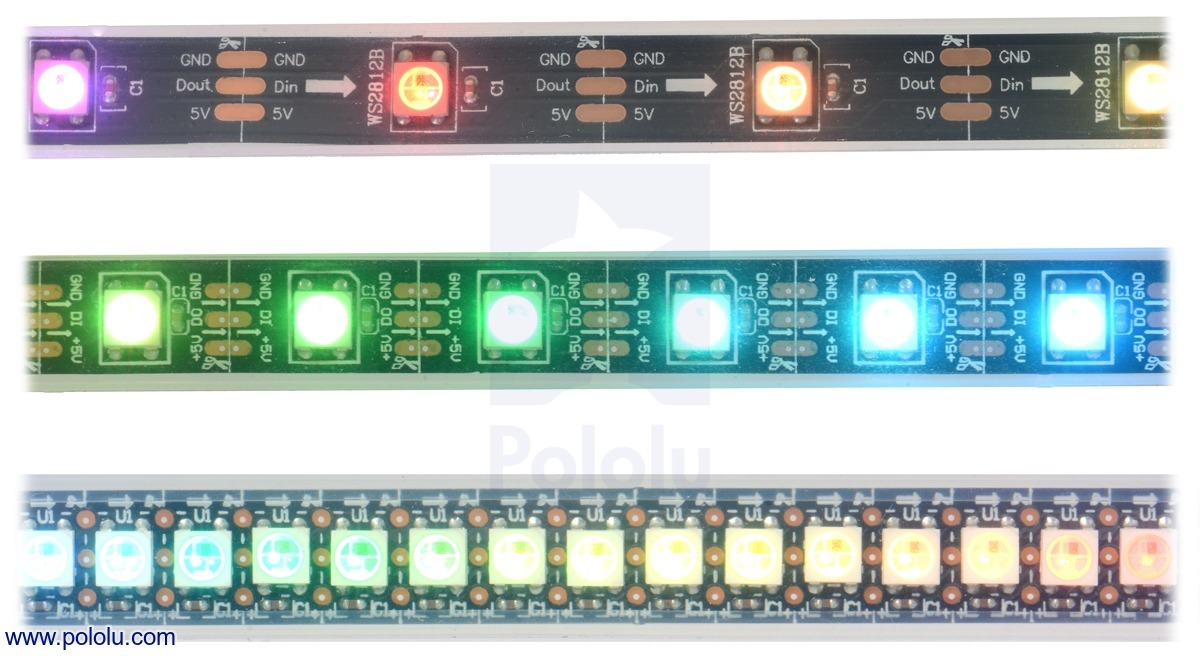
\includegraphics[height=0.35\textwidth, width=\textwidth]{LED.jpg}
\caption{A closer look at the Pololu LED strip [7]}
\end{figure}


\subsection{Challenges}
Most of my actual challenges came from working with the robot. Mainly this had to do with the specifications of the serial connection: whereas the specifications I read online said to use \texttt{`/dev/ttyACM0'} for port and 9600 for baud rate, the robots in the lab use \texttt{`/dev/ttyUSB1'} and 115200, respectively. Thus most of my actual "bugs" that I spent were working on were due to hardware issues, rather than software, leading me to waste a lot of time.\\
\indent Another major issue that I ran into was working with Python. As virtually all of the functional weather APIs didn't provide support for C++, I was essentially forced to use Python for implementing this project. As I didn't have any prior experience with Python before this project, most of the time that I had to spend on this project went to learning basic Python. Thus I was not able to implement most of the extra things that I wanted to do in my proposal, as I was heavily delayed by learning Python. Just getting the basic Python code to work with the Arduino and serial took a lot more time than expected, as I had never really worked with communication between devices before either. Finally, I never used server requests before this, so I had to learn how to obtain information from the Internet in a program without the use of a crawler.


\section{Conclusion and Future Work}

\subsection{Conclusion}
In conclusion, I was able to accomplish my goal of using the LEDs to present the temperatures. Most of my difficulties came from using things that I was unfamiliar with, such as Python, server requests, and serial communication. Thus, I managed to learn a lot while working on this project, and ultimately got it to work. However, there are a lot of improvements that can be made for the code, as well as future extensions that can be built upon it as well.

\subsection{Future Work}
\subsubsection{Improvements}
The primary future work that should be done on this project is removing all of the limitations from the current implementation. Updating the Python code can possibly done by using a while loop. Assuming that the users will always want the code to be running and the forecast updating, most of the code for retrieving and sending the information can be put in a \texttt{while(true)} loop. In order to prevent the loop from instantly reaching the API's request maximum, a \texttt{time.sleep()} statement can be inserted so that the loop waits for certain periods of time before looping. Improvements upon the API are more limited; as this isn't something that the user can directly control and have to rely on outside sources for. However, I think that in a given normal situation, 500 requests per day should be more than enough (ending up at about one request per 3 minutes). Finally, localization can easily be improved by creating a prompt for the user in the Python code. A parser will have to be created for the user's input to analyze what city, state, country is inputted, and then the URL will have to be properly formatted in order to properly handle this input. However, this should not be too time-consuming of a project, and with time and testing is very doable.\\
\indent The colors for the LEDs might be a more difficult problem. As RGB can be largely variable in what values lead to what colors, a different color system may have to be used to allow for easy scaling between blue and red. As for partitioning, I did not have the time to thoroughly investigate why there had to be twelve groups, so there might be other possibilities. If there are alternatives available and code in the framework that allows for the user to easily decide their partitions based on which LED they are using, then this should be used to make the code more portable. Finally, I would imagine that this project can be imported to ROS if given enough knowledge about Python and its use in ROS. As I was struggling to finish the project using pure Python, I was unable to get this. However, with enough time using ROS in Python and better understanding of how serial communication would work in ROS, this would be doable. Also, I do not actually know if Arduino is supported by ROS, so running the Arduino code separately might be a requirement anyway.
\subsubsection{Extensions}
The main future work that can stem from this project are extensions, especially in adding more information. Assuming that the LEDs have to be partitioned into twelve separate groups, up to four categories of information can be given presented per hour. This is because a white light was used to distinguish the different hours (since there are sixty lights per LED strips, five LEDs are used per group, or four informative). Whereas the first can be used for temperatures, the second can be used for precipitation, the third for possible emergencies, etc.: whatever information most pertinent to the geographical location can be used.


\section{References}

[1] https://www.cs.utexas.edu/$\sim$larg/bwi\_scavenger/images/home\_1.jpg\\ \relax
[2] https://www.pololu.com/picture/view/0J3842\\ \relax
[3] https://www.wunderground.com/weather/api/\\ \relax
[4] https://github.com/pololu/pololu-led-strip-arduino\\ \relax
[5] https://dwechsler.wordpress.com/2012/03/13/how-to-programmatically-retrieve-weather-data/\\ \relax
[6] https://stackoverflow.com/questions/24074914/python-to-arduino-serial-read-write\\ \relax
[7] https://www.pololu.com/picture/view/0J5801


\end{document}